\chapter{Important New Developments in Arabographic Optical Character Recognition (OCR)}
\chaptermark{Arabic OCR}
\thispagestyle{empty}
\vfill
This chapter has been published as \fullcite{kiessling2017important}
\newpage
\nocite{soa0}
\nocite{soa1}
\nocite{soa2}
\nocite{soa3}
\nocite{soa4}
\nocite{soa5}
\nocite{soa6}

\section{Introduction}

\subsection{Summary of Results of OpenITI’s OCR}

The OpenITI team\footnote{The co-PIs of the Islamicate Texts Initiative (ITI)
are Sarah Bowen Savant (Aga Khan University, London), Maxim G. Romanov (Leipzig
University), and Matthew Thomas Miller (Roshan Institute for Persian Studies,
University of Maryland, College Park).} building on the foundational
open-source OCR work of the Leipzig University’s (LU) Alexander von Humboldt
Chair for Digital Humanities—has achieved Optical Character Recognition (OCR)
accuracy rates for classical Arabic-script texts in the high nineties. These
numbers are based on our tests of seven different Arabic-script texts of
varying quality and typefaces, totaling over 7,000 lines (~400 pages, 87,000
words; see table~\ref{tab:soa_tab1} for full details). These accuracy rates not
only represent a distinct improvement over the actual\footnote{Proprietary OCR
programs for Persian and Arabic (e.g., Sakhr’s Automatic Reader, ABBYY
Finereader, Readiris) over-promise the level of accuracy they deliver in
practice when used on classical texts. These companies claim that they provide
accuracy rates in the high 90 percentages (e.g., Sakhr claims 99.8\% accuracy
for high-quality documents). This may be the case for texts with simplified
typeset and no short vowels; however, our tests of ABBYY Finereader and
Readiris on high-quality scans of classical texts turned out accuracy rates of
between 65\% and 75\%.  Sakhr software was not available to us, as the
developers offer no trial versions and it is the most expensive commercial OCR
solution for Arabic.  Moreover, since these programs are not open-source and
offer only limited trainability (and created training data cannot be reused),
their costs are prohibitive for most students and scholars and they cannot be
modified according to the interests and needs of the academic community or the
public at large. Most importantly, they have no web interfaces that would
enable the production of wider, user-generated collections.} accuracy rates of
the various proprietary OCR options for printed classical Arabic-script texts,
but, equally important, they are produced using an open-source OCR software
called Kraken (developed by Benjamin Kiessling, LU), thus enabling us to make
this Arabic-script OCR technology freely available to the broader Islamic,
Persian, and Arabic Studies communities in the near future. In the process we
also generated over 7,000 lines of “gold standard” (double-checked) data that
can be used by others for Arabic-script OCR training and testing
purposes.\footnote{This gold standard data is available at:
\url{https://github.com/OpenArabic/OCR_GS_Data}.}


\subsection{OCR and its Importance for Islamicate Studies Fields}

Although there is a wealth of digital Persian and Arabic texts currently
available in various open-access online repositories,\footnote{Collecting and
rendering these texts useful for computational textual analysis (through, for
example, adding scholarly metadata and making them machine-actionable) is a
somewhat separate but deeply interrelated project that OpenITI is currently
working on as well.} these collections still need to be expanded and
supplemented in some important ways. OCR software is critical for this broader
task of expanding the range of digital texts available to scholars for
computational analysis. OCR programs, in the simplest terms, take an image of a
text, such as a scan of a print book, and extract the text, converting the
image of the text into a digital text that then can be edited, searched,
computationally analyzed, etc.   

The specific type of OCR software that we employed in our tests is an
open-source OCR program called Kraken, which was developed by Benjamin
Kiessling at Leipzig University’s Alexander von Humboldt Chair for Digital
Humanities. Unlike more traditional OCR approaches, Kraken relies on a neural
network—which mimics the way we learn—to recognize letters in the images of
entire lines of text without trying first to segment lines into words and then
words into letters. This segmentation step—a mainstream OCR approach that
persistently performs poorly on connected scripts—is thus completely removed
from the process, making Kraken uniquely powerful for dealing with the diverse
variety of ligatures in connected Arabic script (see section 3.1 for more
technical details).

\begin{table}
\begin{minipage}{\textwidth}
\begin{center}
\caption{Description of data}
\label{tab:soa_tab1}
\renewcommand*{\thefootnote}{\alph{footnote}}
\begin{tabularx}{\textwidth}{lXllllll} \toprule
& & & & \multicolumn{4}{c}{\textbf{Size of data samples}}\\
\cline{5-8}
& \textbf{Book}\footnotemark[1] & \textbf{Quality} & \textbf{Type} & \textbf{Pages} & \textbf{Lines} & \textbf{Words} & \textbf{Chars}\\
\midrule
	\textbf{1} & Ibn al-Faqīh \newline\scriptsize{al-Buldān} & 	  high\footnotemark[2] & training 		& 79 & \num{1466} & \num{16909} & \num{92730}\\
	\textbf{2} & Ibn al-Athīr \newline\scriptsize{al-Kāmil} &  	  high\footnotemark[2] & testing 		& 40 & 794 & \num{12818} & \num{58481}\\
	\textbf{3} & Ibn Qutayba \newline\scriptsize{Adab al-kātib} & high\footnotemark[2] & testing	& 55 & 794 & \num{7848} &  \num{42230}\\
	\textbf{4} & al-Jāḥiẓ \newline\scriptsize{al-Ḥayawān} & 	  high\footnotemark[2] & testing		& 65 & 992 & \num{11870} &  \num{59191}\\
	\textbf{5} & al-Yaʿqūbī \newline\scriptsize{al-Taʿrīkh} & 	  high\footnotemark[2] & testing		& 68 & \num{1050} & \num{13487} & \num{66341}\\
	\textbf{6} & al-Dhahabī \newline\scriptsize{Taʾrīkh al-Islām}  & low\footnotemark[3] & testing	& 50 & \num{1110} & \num{11045} & \num{55047}\\
	\textbf{7} & Ibn al-Jawzī \newline\scriptsize{al-Muntaẓam} &    low\footnotemark[3] & testing		& 50 & 938 & \num{13156} & \num{62574}\\
\midrule
\multicolumn{4}{r}{} & 407 & \num{7144} & \num{87133} & \num{436594}\\
\bottomrule
\end{tabularx}
\end{center}
\renewcommand\footnoterule{}
\footnotetext[1]{For details on the editions, see bibliography}
\footnotetext[2]{300 dpi, grayscale spanned specifically for the purpose of testing with ideal parameters}
\footnotetext[3]{200 dpi, black-and-white, pre-binarized, both downloaded from \url{http://www.archive.org} (via \url{http://waqfeya.org})}
\end{minipage}
\end{table}

\section{Initial OCR Tests}

We began our experiments by using Kraken to train a model\footnote{“Training a
model” is a general term used in machine learning for training a program to
recognize certain patterns in data. In the context of OCR work, it refers to
teaching the OCR software to recognize a particular script or typeface—a
process that only requires time and computing power. In our case, this process
required 1 computer core and approximately 24 hours.} on
high-quality\footnote{“High quality” here means 300 dpi, color or grayscale
images. Before the actual process of OCR, these images must be
binarized—converted into black-and-white images; if binarization is not
performed properly, a lot of information is lost from an image, negatively
affecting the accuracy of the OCR process. For this reason, for best results,
one should avoid using pre-binarized images.} scans of \textasciitilde1,000 lines of
Ibn al-Faqīh’s al-Buldān (work \#1). We first generated training data (line
transcriptions) for all of these lines, double checked them (creating so-called
“gold standard” data), trained the model, and, finally,
tested its ability to accurately recognize and extract the text. The results
were impressive, reaching 97.56\% accuracy for the entire text and an even more
impressive 99.68\% accuracy rate on the Arabic script alone (i.e., when errors
related to punctuation and spaces were removed from consideration; such
non-script errors are easy to fix in the post-correction phase and, in many
cases, this correction process for non-script errors can be automated). See
table~\ref{tab:soa_tab2}, row \#1 for full details.\footnote{We have also experimented with the
internal configuration of our models: more extensive models, containing 200
nodes in the hidden middle layer, showed slightly better accuracy in most cases
(works \#4-5 were an exception to this pattern), but it took twice as long to
train and the OCR process using the larger model also takes more time.}

\begin{table}[h!]
\begin{minipage}{\textwidth}
\begin{center}
\caption{Accuracy rates in test of our custom model}
\label{tab:soa_tab2}
\renewcommand*{\thefootnote}{\alph{footnote}}
	\begin{tabularx}{\textwidth}{lp{2.2cm}XXXXXX} \toprule
& & & & \multicolumn{4}{c}{\textbf{Character accuracy}}\\
\cline{5-8}
& \textbf{Book}\footnotemark[1] & \textbf{Quality} & \textbf{Type} & \textbf{Size 100} & \textbf{Ar}\footnotemark[2] & \textbf{Size 200} & \textbf{Ar}\footnotemark[2]\\
\midrule
\textbf{1} & Ibn al-Faqīh \newline\scriptsize{al-Buldān} & 	  high\footnotemark[3] & training & 95.88\% & 99.68\% & 97.56\% & 99.68\%\\
\textbf{2} & Ibn al-Athīr \newline\scriptsize{al-Kāmil} &  	  high\footnotemark[3] & testing & 85.78\% & 90.90\% & 87.18\% & 90.56\%\\
\textbf{3} & Ibn Qutayba \newline\scriptsize{Adab al-kātib} & high\footnotemark[3] & testing	& 75.28\% & 87.67\% & 74.03\% & 87.90\% \\
\textbf{4} & al-Jāḥiẓ \newline\scriptsize{al-Ḥayawān} & 	  high\footnotemark[3] & testing & 69.03\% & 72.78\% & 68.32\% & 71.87\%\\
\textbf{5} & al-Yaʿqūbī \newline\scriptsize{al-Taʿrīkh} & 	  high\footnotemark[3] & testing & 78.78\% & 83.42\% & 78.28\% & 81.85\%\\
\textbf{6} & al-Dhahabī \newline\scriptsize{Taʾrīkh al-Islām}  & low\footnotemark[4] & testing	& 92.19\% & 97.54\% & 94.42\% & 97.61\%\\
\textbf{7} & Ibn al-Jawzī \newline\scriptsize{al-Muntaẓam} &    low\footnotemark[4] & testing & 90.40\% & 97.39\% & 92.26\% & 97.80\%\\
\bottomrule
\end{tabularx}
\end{center}
\renewcommand\footnoterule{}
\footnotetext[1]{For details on the editions, see bibliography}
\footnotetext[2]{Performance on Arabic only (excluding punctuation, spaces and numerals}
\footnotetext[3]{300 dpi, grayscale spanned specifically for the purpose of testing with ideal parameters}
\footnotetext[4]{200 dpi, black-and-white, pre-binarized, both downloaded from \url{http://www.archive.org} (via \url{http://waqfeya.org})}
\end{minipage}
\end{table}

These numbers were so impressive that we decided to expand our study and use
the model built on the text of Ibn al-Faqīh’s al-Buldān (work \#1) to OCR six
other texts. We deliberately selected texts that were different from Ibn
al-Faqīh’s original text in terms of both their Arabic typeface, editorial
orthographic conventions, and image quality. These texts represent at least two
different typefaces (within which there are noticeable variations of font,
spacing, and ligature styles), and four of the texts were high-quality scans
while the other two were low-quality scans downloaded from
\url{www.archive.org} (via \url{http://waqfeya.com/}).\footnote{“Low-quality”
here means 200 dpi, black and white, pre-binarized images. In short, the
standard quality of most scans available on the internet, which are the product
of scanners that prioritize smaller size and speed of scanning for online
sharing (i.e., in contrast to high-quality scans that are produced for
long-term preservation). “Pre-binarized” means that the  images were converted
to black and white during the scanning process, ostensibly for size reduction,
resulting in some degradation of quality.}

When looking at the results in table~\ref{tab:soa_tab2}, it is important that the reader notes
that works \#2-7 are “testing” data. That is, these accuracy results were
achieved by utilizing a model built on the text of work \#1 to perform OCR on
these other texts. For this reason it is not surprising that the accuracy rates
for works \#2-5 are not as high as the accuracy rates for the training text,
work \#1. The point that is surprising is that the use of the work \#1-based
model on the low quality scans of works \#6-7 achieved a substantially higher
accuracy rate (97.61\% and 97.8\% respectively on their Arabic script alone) than
on the high-quality scans of works \#2-5. While these higher accuracy rates for
works \#6-7 are the result of a closer affinity between their typefaces and that
of work \#1, it also indicates that the distinction between high-  and
low-quality images is not as important for achieving high accuracy rates with
Kraken as we initially believed. In the future, this will help reduce
substantially both the total length of time it takes to OCR a work and the
barriers to entry for researchers wanting to OCR the low-quality scans they
already possess.

\begin{table}[h!]
\begin{center}
\caption{Ligature variations in typefaces. The table highlights only a few
	striking differences and is not meant to be comprehensive; examples
	similar to those of the main text are "greyed out."}
\label{tab:soa_tab3}
\renewcommand*{\thefootnote}{\alph{footnote}}
	\begin{tabularx}{\textwidth}{Xp{0.16\textwidth}ccp{0.06\textwidth}ccccc} \toprule
\textbf{Book} & & & & & & & & \\
\midrule
\textbf{1} & Ibn al-Faqīh \newline\scriptsize{al-Buldān} & \raisebox{-0.5\height}{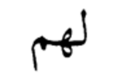
\includegraphics[width=0.06\textwidth]{images/crops/row-1-col-1.png}} 
							 & \raisebox{-0.5\height}{
\includegraphics[width=0.06\textwidth]{images/crops/row-1-col-2.png}}
							 & \raisebox{-0.5\height}{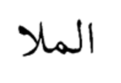
\includegraphics[width=0.06\textwidth]{images/crops/row-1-col-3.png}}
							 & \raisebox{-0.5\height}{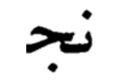
\includegraphics[width=0.06\textwidth]{images/crops/row-1-col-4.png}}
							 & \raisebox{-0.5\height}{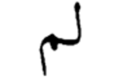
\includegraphics[width=0.06\textwidth]{images/crops/row-1-col-5.png}}
							 & \raisebox{-0.5\height}{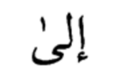
\includegraphics[width=0.06\textwidth]{images/crops/row-1-col-6.png}}
							 & \raisebox{-0.5\height}{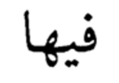
\includegraphics[width=0.06\textwidth]{images/crops/row-1-col-7.png}}
							 & \raisebox{-0.5\height}{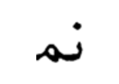
\includegraphics[width=0.06\textwidth]{images/crops/row-1-col-8.png}}
							 \\
\textbf{2} & Ibn al-Athīr \newline\scriptsize{al-Kāmil} & \raisebox{-0.5\height}{
\includegraphics[width=0.06\textwidth]{images/crops/row-2-col-1.png}} 
							& \raisebox{-0.5\height}{
\includegraphics[width=0.06\textwidth]{images/crops/row-2-col-2.png}}
							& \raisebox{-0.5\height}{
\includegraphics[width=0.06\textwidth]{images/crops/row-2-col-3.png}}
							& \raisebox{-0.5\height}{
\includegraphics[width=0.06\textwidth]{images/crops/row-2-col-4.png}}
							& \raisebox{-0.5\height}{
\includegraphics[width=0.06\textwidth]{images/crops/row-2-col-5.png}}
							& \raisebox{-0.5\height}{
\includegraphics[width=0.06\textwidth]{images/crops/row-2-col-6.png}}
							& \raisebox{-0.5\height}{
\includegraphics[width=0.06\textwidth]{images/crops/row-2-col-7.png}}
							& \raisebox{-0.5\height}{
\includegraphics[width=0.06\textwidth]{images/crops/row-2-col-8.png}}
							\\
\textbf{3} & Ibn Qutayba \newline\scriptsize{Adab al-kātib} & \raisebox{-0.5\height}{
\includegraphics[width=0.06\textwidth]{images/crops/row-2-col-1.png}} 
							    & \raisebox{-0.5\height}{
\includegraphics[width=0.06\textwidth]{images/crops/row-2-col-2.png}}
							    & \tiny{not present}
							    & \raisebox{-0.5\height}{
\includegraphics[width=0.06\textwidth]{images/crops/row-2-col-4.png}}
							    & \raisebox{-0.5\height}{
\includegraphics[width=0.06\textwidth]{images/crops/row-2-col-5.png}}
							    & \raisebox{-0.5\height}{
\includegraphics[width=0.06\textwidth]{images/crops/row-2-col-6.png}}
							    & \raisebox{-0.5\height}{
\includegraphics[width=0.06\textwidth]{images/crops/row-2-col-7.png}}
							    & \raisebox{-0.5\height}{
\includegraphics[width=0.06\textwidth]{images/crops/row-2-col-8.png}}
							    \\
\textbf{4} & al-Jāḥiẓ \newline\scriptsize{al-Ḥayawān} & \raisebox{-0.5\height}{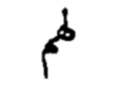
\includegraphics[width=0.06\textwidth]{images/crops/row-4-col-1.png}} 
						      & \raisebox{-0.5\height}{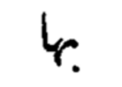
\includegraphics[width=0.06\textwidth]{images/crops/row-4-col-2.png}}
						      & \raisebox{-0.5\height}{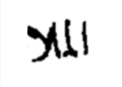
\includegraphics[width=0.06\textwidth]{images/crops/row-4-col-3.png}}
						      & \raisebox{-0.5\height}{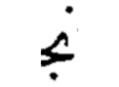
\includegraphics[width=0.06\textwidth]{images/crops/row-4-col-4.png}}
						      & \raisebox{-0.5\height}{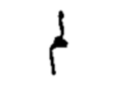
\includegraphics[width=0.06\textwidth]{images/crops/row-4-col-5.png}}
						      & \raisebox{-0.5\height}{
\includegraphics[width=0.06\textwidth]{images/crops/row-4-col-6.png}}
						      & \raisebox{-0.5\height}{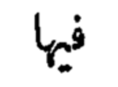
\includegraphics[width=0.06\textwidth]{images/crops/row-4-col-7.png}}
						      & \raisebox{-0.5\height}{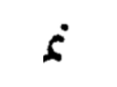
\includegraphics[width=0.06\textwidth]{images/crops/row-4-col-8.png}}
						      \\
\textbf{5} & al-Yaʿqūbī \newline\scriptsize{al-Taʿrīkh}& \raisebox{-0.5\height}{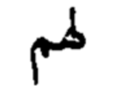
\includegraphics[width=0.06\textwidth]{images/crops/row-5-col-1.png}}
						       & \raisebox{-0.5\height}{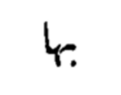
\includegraphics[width=0.06\textwidth]{images/crops/row-5-col-2.png}}
						       & \raisebox{-0.5\height}{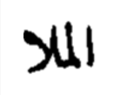
\includegraphics[width=0.06\textwidth]{images/crops/row-5-col-3.png}}
						       & \raisebox{-0.5\height}{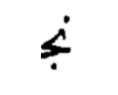
\includegraphics[width=0.06\textwidth]{images/crops/row-5-col-4.png}}
						       & \raisebox{-0.5\height}{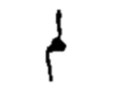
\includegraphics[width=0.06\textwidth]{images/crops/row-5-col-5.png}}
						       & \raisebox{-0.5\height}{
\includegraphics[width=0.06\textwidth]{images/crops/row-5-col-6.png}}
						       & \raisebox{-0.5\height}{
\includegraphics[width=0.06\textwidth]{images/crops/row-5-col-7.png}}
						       & \raisebox{-0.5\height}{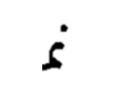
\includegraphics[width=0.06\textwidth]{images/crops/row-5-col-8.png}}\\
\textbf{6} & al-Dhahabī \newline\scriptsize{Taʾrīkh al-Islām}& \raisebox{-0.5\height}{
\includegraphics[width=0.06\textwidth]{images/crops/row-6-col-1.jpg}}
							     & \raisebox{-0.5\height}{
\includegraphics[width=0.06\textwidth]{images/crops/row-6-col-2.jpg}}
							     & \tiny{not present}
							     & \raisebox{-0.5\height}{
\includegraphics[width=0.06\textwidth]{images/crops/row-6-col-4.jpg}}
							     & \raisebox{-0.5\height}{
\includegraphics[width=0.06\textwidth]{images/crops/row-6-col-5.jpg}}
							     & \raisebox{-0.5\height}{
\includegraphics[width=0.06\textwidth]{images/crops/row-6-col-6.jpg}}
							     & \raisebox{-0.5\height}{
\includegraphics[width=0.06\textwidth]{images/crops/row-6-col-7.jpg}}
							     & \raisebox{-0.5\height}{
\includegraphics[width=0.06\textwidth]{images/crops/row-6-col-8.jpg}}\\
\textbf{7} & Ibn al-Jawzī \newline\scriptsize{al-Muntaẓam}& \raisebox{-0.5\height}{
\includegraphics[width=0.06\textwidth]{images/crops/row-7-col-1.png}}
							  & \raisebox{-0.5\height}{
\includegraphics[width=0.06\textwidth]{images/crops/row-7-col-2.png}}
							  & \tiny{not present}
							  & \raisebox{-0.5\height}{
\includegraphics[width=0.06\textwidth]{images/crops/row-7-col-4.png}}
							  & \raisebox{-0.5\height}{
\includegraphics[width=0.06\textwidth]{images/crops/row-7-col-5.png}}
							  & \raisebox{-0.5\height}{\includegraphics[width=0.06\textwidth]{images/crops/row-7-col-6.png}}
							  & \raisebox{-0.5\height}{\includegraphics[width=0.06\textwidth]{images/crops/row-7-col-7.png}}
							  & \raisebox{-0.5\height}{\includegraphics[width=0.06\textwidth]{images/crops/row-7-col-8.png}}\\
\bottomrule
\end{tabularx}
\end{center}
\end{table}

(the table highlights only a few striking differences and is not meant to be comprehensive;
examples similar to those of the main text are “greyed out”)  

The decreased accuracy results for works \#2-5 are explainable by a few factors:

\begin{enumerate}
	\item The typeface of works \#4-5 is different than work \#1 and it utilizes a number of ligatures that are not present in the typeface of work \#1 (for examples, see table~\ref{tab:soa_tab3} above). 
	\item The typefaces of work \#2-3 are very similar to that of \#1, but they both have features that interfere with the \#1-based model. \#2 actually uses two different fonts, and the length of connections—kashīdas—between letters vary dramatically (0.3 kashīda to 2 kashīdas and everything in between), which is not the case with \#1, where letter spacing is very consistent. 
	\item The text of work \#3 is highly vocalized—it has more ḥarakāt than any other texts in the sample (and especially in comparison with the model work \#1).
	\item The text of work \#3 also has very complex and overabundant punctuation with highly inconsistent spacing. 
\end{enumerate}

Our \#1-based model could not completely handle these novel features in the texts of works \#2-5 because it was not trained to do so. As the results in table~\ref{tab:soa_tab4} of the following section show, new models can be trained to handle these issues successfully.

\begin{table}[h!]
\begin{minipage}{\textwidth}
\begin{center}
\caption{Accuracy rates in text-specific models}
\label{tab:soa_tab4}
\renewcommand*{\thefootnote}{\alph{footnote}}
\begin{tabularx}{\textwidth}{lXllll} \toprule
& & & & \multicolumn{2}{c}{\textbf{Character accuracy}}\\
\cline{5-6}
& \textbf{Book}\footnotemark[1] & \textbf{Quality} & \textbf{Type} & \textbf{Size 100} & \textbf{Ar}\footnotemark[2]\\
\midrule
\textbf{2} & Ibn al-Athīr \scriptsize{al-Kāmil} &  	  high\footnotemark[3] & testing & 93.79\% & 97.71\%\\
\textbf{3} & Ibn Qutayba \scriptsize{Adab al-kātib} & high\footnotemark[3] & testing & 89.30\% & 98.47\%\\
\textbf{4} & al-Jāḥiẓ \scriptsize{al-Ḥayawān} & 	  high\footnotemark[3] & testing & 94.87\% & 97.59\%\\
\textbf{5} & al-Yaʿqūbī \scriptsize{al-Taʿrīkh} & 	  high\footnotemark[3] & testing & 96.81\% & 99.18\% \\
\bottomrule
\end{tabularx}
\end{center}
\renewcommand\footnoterule{}
\footnotetext[1]{For details on the editions, see bibliography}
\footnotetext[2]{Performance on Arabic only (excluding punctuation, spaces and numerals}
\footnotetext[3]{300 dpi, grayscale spanned specifically for the purpose of testing with ideal parameters}
\end{minipage}
\end{table}

\section{Round \#2 Tests: Training New Models}

The most important advantage of Kraken is that its workflow allows one to train
new models relatively easily, including text-specific ones. In a nutshell, the
process of training requires a transcription of approximately 800 lines (the
number will vary depending on the complexity of the typeface) aligned with
images of these lines as they appear in the printed edition. The training
itself takes 12-24 hours and is performed by a machine without human
involvement; multiple models can be trained simultaneously. Kraken includes
tools for the production of transcription forms (see figure~\ref{fig:soa_1} below); the data
supplied through these forms is then used to train a new model. (Since there
are a great number of Arabic-script texts that have already been converted into
digital texts, one can use these as the base texts to fill in the forms more
quickly—i.e., instead of typing the transcription—and then double-check them
for accuracy; this was what we did, and it saved us a lot of time.)

\begin{figure}
        \centering
        \includegraphics[width=0.9\textwidth]{images/image10.png}
	\caption{Kraken’s Transcription Interface}
	\label{fig:soa_1}
\end{figure}


The importance of Kraken’s ability to quickly train new models is illustrated
clearly by texts such as works \#2-5 . When using the model built on work \#1 in
our initial round of testing, we were only able to achieve accuracy rates
ranging from the low seventies to low nineties on these texts (see table~\ref{tab:soa_tab2}).
However, when we trained models on works \#2-5 specifically in our second round
of testing, the accuracy rates for these texts substantially improved, reaching
into the high nineties (see full results in table~\ref{tab:soa_tab4} above). The accuracy
results for work \#5, for example, improved from 83.42\% on Arabic script alone
in our first work \#1-based model tests to 99.18\% accuracy when we trained a
mode on this text. The accuracy rates for works \#2-4 similarly improved,
increasing from 90.90\% to 97.71\% , 87.90\% to 98.47\%, from 72.78\% to
97.59\%, respectively. (See Appendix for the accuracy rates of these new models
on all other texts as well.) These accuracy rates for Arabic-script recognition
are already high, but we actually believe that they can be improved further
with larger training data sets.

Although the process of training a new model for a new text/typeface does
require some effort, the only time-consuming component is the generation of
\textasciitilde800 lines of gold standard training data. As we develop the OpenITI OCR
project we will address the issue of the need for multiple models through a
two-pronged strategy. First, we will try to train a general model, periodically
adding new features that the model has not “seen” before. Secondly, we will
train individual models for distinct typefaces and editorial styles (which
sometimes vary in their use of vocalization, fonts, spacing, and punctuation),
producing a library of OCR models that gradually will cover all major typefaces
and editorial styles used in modern Arabic-script printing. There certainly are
numerous Arabic-script typefaces and editorial styles that have been used
throughout the last century and a half of Arabic-script printing, but
ultimately the number is finite and definitely not so numerous as to make it
impossible to create models for each over the long term.  


\section{Conclusions and Next Steps for the OpenITI OCR Project}

The two rounds of testing presented here indicate that with a fairly modest
amount of gold standard training data (\textasciitilde800–1,000 lines) Kraken is
consistently able to produce OCR results for Arabic-script documents that
achieve accuracy rates in the high nineties. In some cases, such as works
\#6-7, achieving OCR accuracy rates of up to 97.5\% does not even require
training a new model on that text. However, in other cases, such as works
\#2-5, achieving high levels of OCR accuracy does require training a model
specific to that typeface, and, in some select cases of texts with similar
typefaces but different styles of vocalization, font variations, and
punctuation patterns (e.g., works \#2-3), training a model for the
peculiarities of a particular edition.

\begin{figure}
        \centering
        \includegraphics[width=0.9\textwidth]{images/image3.png}
	\caption{Web-based OCR pipeline flowchart}
	\label{fig:soa_2}
\end{figure}
  

In the near future we are planning to develop a user-friendly web-interface for
the generation of new training data and the post-correction of the OCR output
(see figure~\ref{fig:soa_2} above). Data supplied by users will allow us to train new
models. It should be stressed that training edition-specific models is quite
valuable, as there is a number of multivolume books—often with over a dozen
volumes per text—that need to be converted into proper digital editions. In the
long term, we are also planning to train models for other Islamicate languages
(Ottoman Turkish, Urdu, Syriac,\footnote{Together with George Kiraz (Gorgias
Press, Editor-in-Chief; Rutgers University, Visiting Scholar), we have most
recently tested Kraken on Syriac texts, achieving comparable accuracy rates of
95.17–99.09\%.} etc.). Our hope is that an easy-to-use and effective OCR
pipeline will allow us, all,collectively to significantly enrich our collection
of digital Persian and Arabic texts and thereby enable us to understand better
the cultural heritage of the Middle East as reflected in its literary
traditions.


\section{The Technical Details: Kraken and its OCR Method}

Kraken is the open-source OCR software that we used in our tests. Developed by
Benjamin Kiessling at UL’s Alexander von Humboldt Chair for Digital Humanities,
Kraken is a “fork”\footnote{“Fork” is a computer-science term for a new
independent development that builds on an existing software.} of the
unmaintained ocropus package\footnote{For details, see:
\url{https://github.com/tmbdev/ocropy} and
\url{https://en.wikipedia.org/wiki/OCRopus}.} combined with the CLSTM neural
network library.\footnote{See: \url{https://github.com/tmbdev/clstm}.} Kraken
represents a substantial improvement over the ocropus package: its performance
is drastically better, it supports right-to-left scripts and combined LTR/RTL
(BiDi) texts, and it includes a rudimentary transcription interface for offline
use.

The OCR method that powers Kraken is based on a long short-term memory
\cite{hochreiter1997long} recurrent neural network utilizing the Connectionist
Temporal Classification objective function (\cite{graves2006connectionist}, as
elaborated in \cite{breuel2013high}). In contrast to other systems requiring
character level segmentation before classification, it is uniquely suited for
the recognition of connected Arabographic scripts because the objective
function used during training is geared towards assigning labels—i.e.,
characters/glyphs—to regions of unsegmented input data. 

The system works on unsegmented data both during training and recognition—its
base unit is a text line (line recognizer). For training, a number of printed
lines have to be transcribed using a simple HTML transcription interface (see
figure~\ref{fig:soa_1} above). The total amount of training data (i.e., line image-text
pairs) required may vary depending on the complexity of the typeface and number
of glyphs used by the script. Acquisition of training data can be optimized by
line-wise alignment of existing digital editions with printed lines, although
even wholesale transcription is a faster and relatively unskilled task in
comparison to training data creation for other systems such as
tesseract.\footnote{See: \url{https://github.com/tesseract-ocr} and
\url{https://en.wikipedia.org/wiki/Tesseract_(software)}.}

Our current models were trained on \textasciitilde1,000 pairs each, corresponding to
\textasciitilde50-60 pages of printed text. Models are fairly typography specific,
the most important factor being fonts and spacing, although some mismatch does
not degrade recognition accuracy substantially (2-5\%).\footnote{For example,
if a glyph is in a slightly different font than the one that the model was
trained on, it may sometimes be misrecognized as another one (or not at all),
thus leading the overall accuracy rate to be slightly lower despite the fact
that most of the other text is recognized correctly.} Thus new training data
for an unknown typeface can be produced by correcting the output from a model
for a similar font—in other words, generating training data for every
subsequent model will require less and less time. Last but not least, it is
also possible to train multi-typeface models by simply combining training data,
albeit some parameter tuning is required to account for the richer typographic
morphology that the neural network must learn.

\section{Acknowledgements}

We would never have been able to complete this work without the help of our
team members at Leipzig University, University of Maryland (College Park), and
Aga Khan University, London. We would also like to thank Elijah Cooke (Roshan
Institute, UMD) for helping us to process the data, Samar Ata (Roshan
Institute, UMD) for generating several sets of high-quality scans for us, and
Layal Mohammad (ISMC, AKU), Mohammad Meqdad (ISMC, AKU), and Fatemeh Shams
(ISMC, AKU) for helping us to generate and double check the training data.
Lastly, we would like to express our gratitude to Gregory Crane (Alexander von
Humboldt Chair for Digital Humanities, LU), Fatemeh Keshavarz (Roshan Institute
for Persian Studies, UMD), and David Taylor (ISMC, AKU) for their guidance and
support of our work. 

\begin{subappendices}
\newpage
\section{Performance of Text-Specific Models}

\begin{table}[H]
\begin{minipage}{\textwidth}
\begin{center}
\caption{Performance of \#2-based model on other texts}
\label{tab:soa_atab1}
\renewcommand*{\thefootnote}{\alph{footnote}}
\begin{tabularx}{\textwidth}{lp{2.2cm}XXXXXX} \toprule
& & & & \multicolumn{4}{c}{\textbf{Character accuracy}}\\
\cline{5-8}
& \textbf{Book}& \textbf{Quality} & \textbf{Type} & \textbf{Size 100} & \textbf{Ar}& \textbf{Size 200} & \textbf{Ar}\\\midrule
\textbf{2} & \textbf{Ibn al-Athīr \newline\scriptsize{al-Kāmil}} &  	  \textbf{high} & \textbf{training} & \textbf{93.79\%} & \textbf{97.71\%} & \textbf{93.58\%} & \textbf{97.59\%}\\
\textbf{3} & Ibn Qutayba \newline\scriptsize{Adab al-kātib} & high& testing	& 82.68\% & 95.72\% & 80.92\% & 94.88\% \\
\textbf{4} & al-Jāḥiẓ \newline\scriptsize{al-Ḥayawān} & 	  high& testing & 71.78\% & 75.16\% & 70.85\% & 74.27\%\\
\textbf{5} & al-Yaʿqūbī \newline\scriptsize{al-Taʿrīkh} & 	  high& testing & 79.67\% & 84.40\% & 78.12\% & 82.21\%\\
\textbf{6} & al-Dhahabī \newline\scriptsize{Taʾrīkh al-Islām}  & low& testing	& 90.68\% & 95.95\% & 90.37\% & 95.78\%\\
\textbf{7} & Ibn al-Jawzī \newline\scriptsize{al-Muntaẓam} &    low& testing & 93.33\% & 98.51\% & 92.96\% & 98.22\%\\
\bottomrule
\end{tabularx}
\end{center}
\end{minipage}
\end{table}

\begin{table}[H]
\begin{minipage}{\textwidth}
\begin{center}
\caption{Performance of \#3-based model on other texts}
\label{tab:soa_atab2}
\renewcommand*{\thefootnote}{\alph{footnote}}
\begin{tabularx}{\textwidth}{lp{2.2cm}XXXXXX} \toprule
& & & & \multicolumn{4}{c}{\textbf{Character accuracy}}\\
\cline{5-8}
& \textbf{Book}& \textbf{Quality} & \textbf{Type} & \textbf{Size 100} & \textbf{Ar}& \textbf{Size 200} & \textbf{Ar}\\\midrule
\textbf{2} & Ibn al-Athīr \newline\scriptsize{al-Kāmil} &  	  high& testing & 83.52\% & 88.56\% & 83.55\% & 88.56\%\\
\textbf{3} & \textbf{Ibn Qutayba \newline\scriptsize{Adab al-kātib}} & \textbf{high}& \textbf{training} & \textbf{89.30\%} & \textbf{98.47\%} & \textbf{89.42\%} & \textbf{98.44\%} \\
\textbf{4} & al-Jāḥiẓ \newline\scriptsize{al-Ḥayawān} & 	  high& testing & 74.82\% & 76.51\% & 74.87\% & 76.65\%\\
\textbf{5} & al-Yaʿqūbī \newline\scriptsize{al-Taʿrīkh} & 	  high& testing & 81.50\% & 84.05\% & 79.81\% & 83.67\%\\
\textbf{6} & al-Dhahabī \newline\scriptsize{Taʾrīkh al-Islām}  & low& testing	& 84.89\% & 93.19\% & 83.08\% & 92.53\%\\
\textbf{7} & Ibn al-Jawzī \newline\scriptsize{al-Muntaẓam} &    low& testing & 87.56\% & 94.21\% & 86.34\% & 93.57\%\\
\bottomrule
\end{tabularx}
\end{center}
\end{minipage}
\end{table}

\begin{table}[H]
\begin{minipage}{\textwidth}
\begin{center}
\caption{Performance of \#4-based model on other texts}
\label{tab:soa_atab3}
\renewcommand*{\thefootnote}{\alph{footnote}}
\begin{tabularx}{\textwidth}{lp{2.2cm}XXXXXX} \toprule
& & & & \multicolumn{4}{c}{\textbf{Character accuracy}}\\
\cline{5-8}
& \textbf{Book}& \textbf{Quality} & \textbf{Type} & \textbf{Size 100} & \textbf{Ar}& \textbf{Size 200} & \textbf{Ar}\\\midrule
\textbf{2} & Ibn al-Athīr \newline\scriptsize{al-Kāmil} &  	  high& testing & 80.23\% & 86.27\% & 82.46\% & 87.48\%\\
\textbf{3} & Ibn Qutayba \newline\scriptsize{Adab al-kātib} & high& testing	& 80.90\% & 91.54\% & 82.61\% & 93.24\% \\
\textbf{4} & \textbf{al-Jāḥiẓ \newline\scriptsize{al-Ḥayawān}} & 	  \textbf{high}& \textbf{training} & \textbf{94.86\%} & \textbf{97.59\%} & \textbf{94.82\%} & \textbf{97.41\%}\\
\textbf{5} & al-Yaʿqūbī \newline\scriptsize{al-Taʿrīkh} & 	  high& testing & 90.91\% & 95.13\% & 91.28\% & 94.71\%\\
\textbf{6} & al-Dhahabī \newline\scriptsize{Taʾrīkh al-Islām}  & low& testing	& 81.93\% & 91.23\% & 83.03\% & 92.22\%\\
\textbf{7} & Ibn al-Jawzī \newline\scriptsize{al-Muntaẓam} &    low& testing & 84.07\% & 93.58\% & 86.26\% & 94.20\%\\
\bottomrule
\end{tabularx}
\end{center}
\end{minipage}
\end{table}

\begin{table}[H]
\begin{minipage}{\textwidth}
\begin{center}
\caption{Performance of \#5-based model on other texts}
\label{tab:soa_atab4}
\renewcommand*{\thefootnote}{\alph{footnote}}
\begin{tabularx}{\textwidth}{lp{2.2cm}XXXXXX} \toprule
& & & & \multicolumn{4}{c}{\textbf{Character accuracy}}\\
\cline{5-8}
& \textbf{Book}& \textbf{Quality} & \textbf{Type} & \textbf{Size 100} & \textbf{Ar}& \textbf{Size 200} & \textbf{Ar}\\ \midrule
\textbf{2} & Ibn al-Athīr \newline\scriptsize{al-Kāmil} &  	  high& testing & 79.80\% & 86.35\% & N/A & N/A\\
\textbf{3} & Ibn Qutayba \newline\scriptsize{Adab al-kātib} & high& testing	& 72.99\% & 82.84\% & N/A & N/A \\
\textbf{4} & al-Jāḥiẓ \newline\scriptsize{al-Ḥayawān} & 	  high& testing & 83.38\% & 87.65\% & N/A & N/A\\
\textbf{5} & \textbf{al-Yaʿqūbī \newline\scriptsize{al-Taʿrīkh}} & 	  \textbf{high} & \textbf{training} & \textbf{96.81\%} & \textbf{99.18\%} & \textbf{N/A} & \textbf{N/A}\\
\textbf{6} & al-Dhahabī \newline\scriptsize{Taʾrīkh al-Islām}  & low& testing	& 82.76\% & 90.65\% & N/A & N/A\\
\textbf{7} & Ibn al-Jawzī \newline\scriptsize{al-Muntaẓam} &    low& testing & 87.71\% & 96.00\% & N/A & N/A\\
\bottomrule
\end{tabularx}
\end{center}
\end{minipage}
\end{table}
\end{subappendices}
%[1] Our logo, Kraken ibn Ocropus, is based on a depiction of an octopus from a manuscript of Kitāb al-ḥashāʾish fī hāyūlā al-ʿilāj al-ṭibbī (Leiden, UB : Or. 289); special thanks to Emily Selove for help with finding an octopus in the depths of the Islamic manuscript tradition.
